% ------------------------------------------------------------------------------
%
% PREAMBLE
%
% ------------------------------------------------------------------------------

\documentclass[12pt, titlepage]{article}


\usepackage{graphicx, amsmath, amssymb, natbib, setspace, sectsty, verbatim, 
		mathrsfs, float}
\usepackage{MnSymbol}
\usepackage{multirow}
\usepackage{bm}
\usepackage[usenames, dvipsnames]{color}
\bibpunct{(}{)}{;}{a}{}{,}
\setlength{\parindent}{3em}
%\parskip = 1.5ex
%\linespread{1.3}
%\onehalfspacing

\pdfpagewidth 8.5in
\pdfpageheight 11in
\setlength{\oddsidemargin}{0.0in} \setlength{\textwidth}{6.5in}
\setlength{\topmargin}{0.15in} \setlength{\textheight}{8.5in}
\setlength{\headheight}{0.0in} \setlength{\headsep}{0.0in}

\usepackage{/mnt/ExtraDrive1/Work/shTex/mymacros}

\providecommand{\norm}[1]{\lVert#1\rVert}
\newcommand{\csection}[1]{\section[#1]{\centering #1 }}
\subsectionfont{\small}
\newcommand{\cye}[1]{\color{yellow!70!black}#1}
\newcommand{\cre}[1]{\color{red!70!black}#1}
\newcommand{\cbl}[1]{\color{blue!70!black}#1}
\newcommand{\cgr}[1]{\color{green!70!black}#1}


% ------------------------------------------------------------------------------
%
% BEGIN DOCUMENT
%
% ------------------------------------------------------------------------------

\begin{document}

\setcounter{equation}{0}
\renewcommand{\theequation}{R.\arabic{equation}}


% ------------------------------------------------------------------------------
%
%                    Section 8.8.3
%                    The wet sulfate desposition data
%
% ------------------------------------------------------------------------------

{\large \flushleft \textbf{8.8.3 The wet sulfate desposition data}}

\vspace{.3cm}

Exploratory data analysis scattered throughout Chapter 3 suggested that it would be wise to transform the wet sulfate deposition data to the square-root scale and to set aside three outliers, yielding a modified dataset that was called the clean wet sulfate deposition data.  Polynomials of orders zero through five were fitted to these modified data by OLS in Section 4.5.3, and summary statistics from these fits suggested that polynomials up to third-order (and possibly higher) were worthy of further consideration.  The analyses presented in Section 4.5.3 also suggested that spatial autocorrelation exists and is isotropic in the residuals from the quadratic fit, but perhaps does not exist in the residuals from the cubic and higher-order fits.

\begin{figure}[H]
  \begin{center}
	    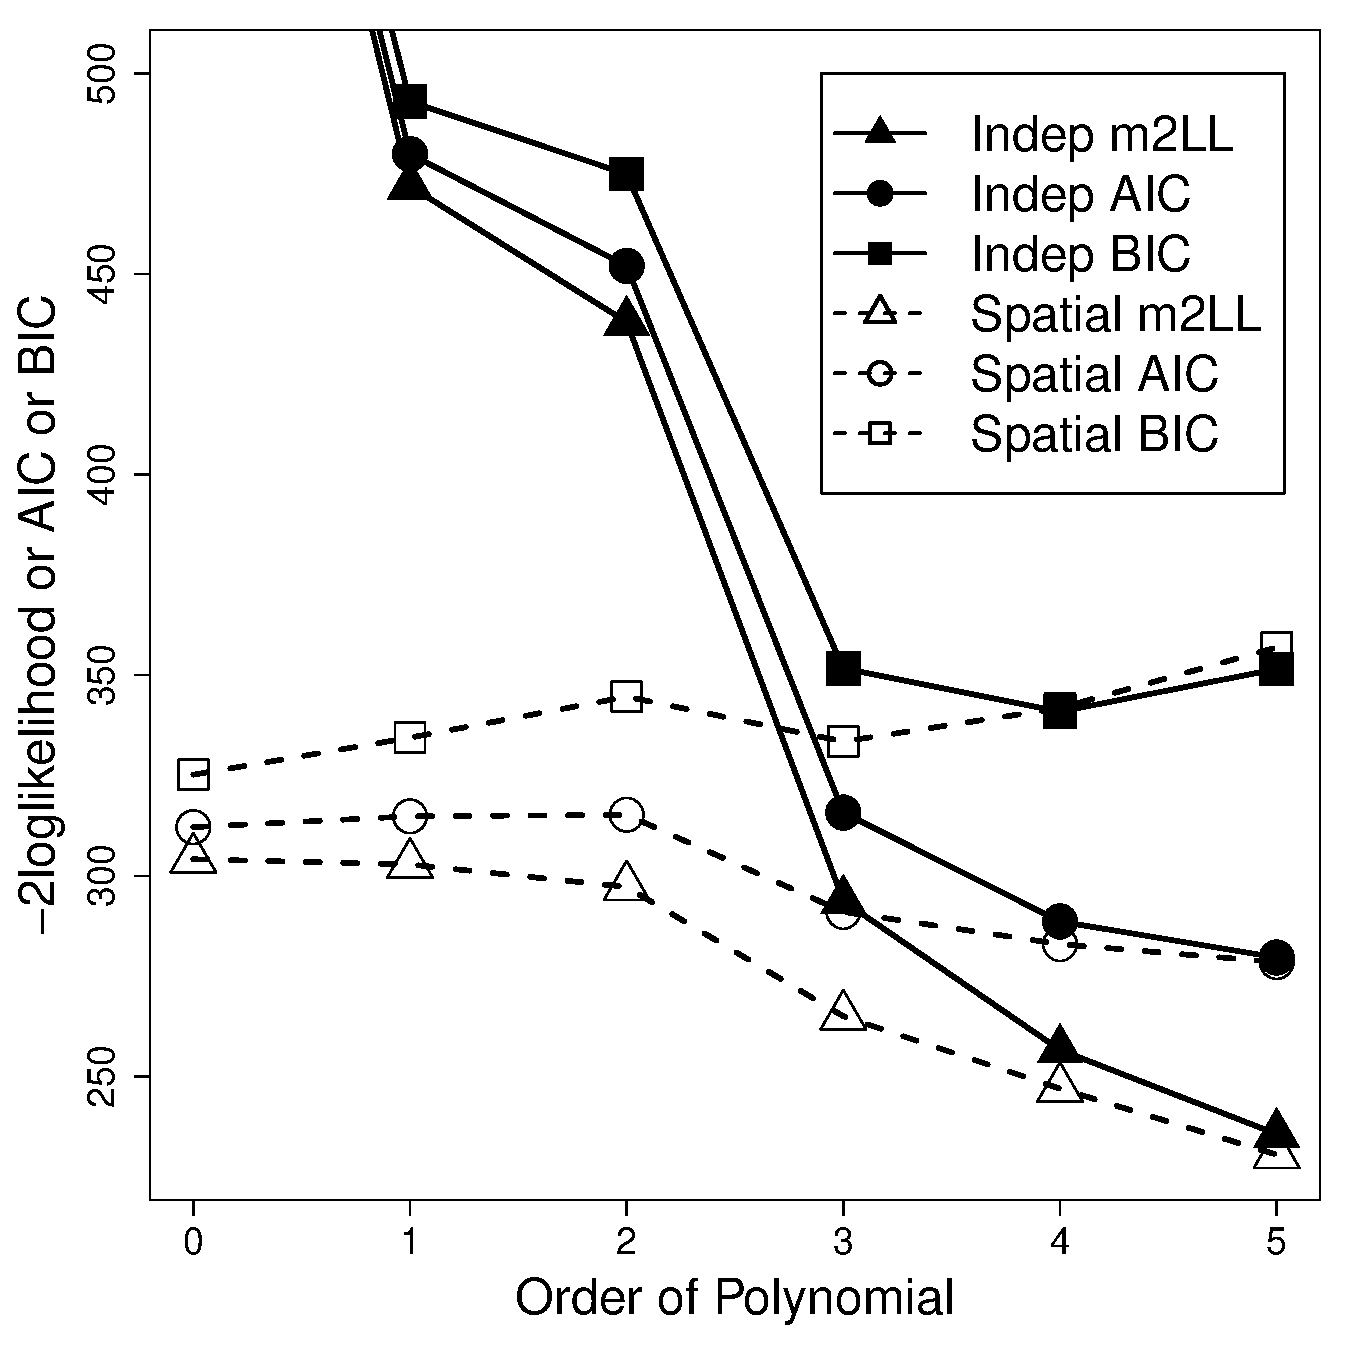
\includegraphics[width=.6\linewidth]{SO4_AIC}
  \end{center}
  \caption{Two times the negative log-likelihood (m2LL, triangles), AIC (circles), and BIC (squares) for polynomial models on the spatial coordinates, for both independent error models (solid lines and solid shapes) and spatial models (dashed line and open shapes). \label{Fig:SO4_AIC}}
\end{figure}

Here, we fit polynomial models to the clean wet sulfate deposition data once again, but this time using likelihood-based methods.  Models having polynomial mean structures up to (and including) order five and having several geostatistical covariance functions were estimated by MLE using the \texttt{R} package \texttt{spmodel}, which also returns AIC and the log-likelihood, from which we computed BIC.  Figure~\ref{Fig:SO4_AIC} shows $-2\log\l(\bar{\boldsymbol{\beta}},\bar{\boldsymbol{\theta}})$ (which we denote as m2LL), AIC, and BIC computed for all polynomial models on the two spatial coordinates from the constant mean model up to a fifth-order polynomial for both independent error models and spatially-autocorrelated error models, where the spatial autocorrelation is an exponential model. Note that m2LL decreases as the order of the polynomial increases, as it must, because the models are nested. AIC and BIC are greater than m2LL due to their respective penalties that depend on the number of parameters and sample size, which is readily seen in Figure~\ref{Fig:SO4_AIC}. 
\begin{figure}[H]
  \begin{center}
	    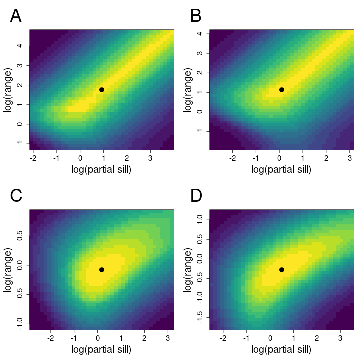
\includegraphics[width=.8\linewidth]{SO4_Viz_m2LL_covParms}
  \end{center}
  \caption{Surface of the restricted log-likelihood for the logarithm of the partial sill ($\log(\theta_{1})$) by the logarithm of the range parameters ($\log(\theta_{2})$ while holding the nugget effect constant at its restricted maximum likelihood estimate. A. Circular model. B. spherical model. C. Gaussian model. D. Gravity model.  The more yellow colors are larger likelihood values, and the bluer colors are smaller likelihood values. The REML estimates are shown as solid black circles. \label{Fig:SO4_psill_range}}
\end{figure} 
For both the independent models and spatial models, AIC generally decreases most rapidly between the 2nd and 3rd orders of the polynomials, and continues to decrease, but more slowly for higher order polynomials. AIC has a reputation for favoring overly complex models, so we also show BIC (Figure~\ref{Fig:SO4_AIC}).  While AIC suggests that the ``best'' model is a 5th order polynomial for both independence and spatial models, BIC suggests that a 4th order polynomial is best if assuming the errors are independent, while BIC suggests that a constant mean model is best when considering spatially autocorrelated models.  We will consider model selection for these data in more detail after we introduce prediction in Chapter 9.

Fitting spatial models is more complicated than fitting models where errors are assumed independent.  One feature of almost all models listed in Table 6.1 is that there is ``correlation'' in the likelihood between $\theta_{1}$, the partial sill, and $\theta_{2}$, the range parameter.  To investigate this, we use REMLE for a constant mean model for the circular, spherical, Gaussian, and gravity models, Figure~\ref{Fig:SO4_psill_range}), which plots the log-likelihood as a function of the logarithms of the range ($\theta_{2}$) and partial sill ($\theta_{1}$) parameters.

In fact, \citet{zhang_inconsistent_2004} shows that estimation of $\theta_{1}$ and $\theta_{2}$ are asymptotically inconsistent, but estimation of their ratio $\theta_{1}/\theta_{2}$ is asymptotically consistent.  This is most apparent in the long ridge in Figure~\ref{Fig:SO4_psill_range}B. There are nearly equal likelihood values all along this ridge, and, in fact, practitioners of geostatistics are well aware that sometimes optimization does not converge as both the range and partial sill increase along this ridge. However, \citet{zhang_inconsistent_2004} also shows that predictions and their standard errors are largely insensitive to the values of $\theta_{1}$ and $\theta_{2}$ themselves, but are sensitive to their ratio.  Thus, it matters little where estimates settle on the ridge seen in Figure~\ref{Fig:SO4_psill_range}B because the ratio remains relatively constant.  Practitioners of geostatistics have also been aware of this for years, and often set a bound on one of these parameters to force convergence, realizing that little changes by letting the range and partial sill continue to increase during optimization.

It is also instructive to look at the likelihood by allowing the partial sill and nugget to vary, while holding the range parameter constant.  The resulting surface for the spherical model shown in Figure~\ref{Fig:SO4_psill_range}B is given in Figure~\ref{Fig:SO4_psill_nugget}. Notice that there is negative correlation between the partial sill and nugget in the likelihood.  This makes sense because there is only so much variation in the data. If we think of the total variance as (nugget + partial sill), then if one goes up, the other must go down, and that is expressed in the likelihood shown in Figure~\ref{Fig:SO4_psill_nugget}.
\begin{figure}[H]
  \begin{center}
	    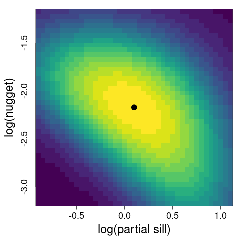
\includegraphics[width=.5\linewidth]{SO4_psillvsnugget}
  \end{center}
  \caption{Likelihood surface for the logarithm of the partial sill, $\log(\theta_{1})$, by the logarithm of the nugget parameter, $\log(\theta_{0})$, while holding the range parameter constant at its restricted maximum likelihood estimate. The REML estimate is shown as a solid black circle. \label{Fig:SO4_psill_nugget}}
\end{figure}

The curvature of the likelihood at the REMLE (or MLE) is approximated by Fisher's Information matrix, which can be used to construct confidence intervals as suggested earlier.  After fitting the model, we can easily compute 
$$
\boldsymbol{F}_{a}{(\boldsymbol{\theta})_{i,j}} = \frac{1}{2}\operatorname{tr}\left(\boldsymbol{\Sigma}^{-1} \frac{\partial \boldsymbol{\Sigma}}{\partial\theta_i}{\boldsymbol{\Sigma}^{-1}}\frac{\partial\boldsymbol{\Sigma}}{\partial\theta_j}\right),
$$
by noting the general form $\boldsymbol{\Sigma} = \theta_{1}\mathbf{R}(\theta_{2}) + \theta_{0}\mathbf{I}$, and hence $\partial \boldsymbol{\Sigma}/ \partial \theta_0 = \mathbf{I}$, $\partial \boldsymbol{\Sigma}/ \partial \theta_1 = \mathbf{R}(\theta_{2})$ and $\partial \boldsymbol{\Sigma}/ \partial \theta_2 = \theta_{1}\mathbf{A}$, where $\mathbf{A}$ is a matrix constructed based on the estimated parameters and distance in $\partial \sigma(r,\boldsymbol{\theta})/\partial \theta_{2}$ (Table 6.1).  For example, if $\mathbf{D}$ is the matrix of all pairwise distances, and we chose an exponential model, then $\mathbf{A} = \mathbf{D}\odot\mathbf{R}/\theta_{2}^{2}$, where $\odot$ is the Hadamard or direct product.  Then the asymptotic standard errors are the square roots of the diagonal of $\boldsymbol{F}^{-1}_{a}{(\boldsymbol{\theta})}$.  We fitted constant mean models with REMLE, and the estimated values of covariance parameters for various autocovariance models, along with their estimated standard errors based on Fisher's Information, are given in Table~\ref{tab:AsySE}.

Another approach is to compute the Hessian matrix of the log-likelihood.  We used \texttt{spmodel} for this as it allowed us to evaluate the log-likelihood for any given value of $\boldsymbol{\theta}$.  We used the \texttt{R} package \texttt{numDeriv} to compute the numeric Hessian, $\mathbf{H}$, at the REMLE, and then an estimator of Fisher's Information is,
$$
\boldsymbol{F}_{n}{(\boldsymbol{\theta})} = -\mathbf{H},
$$
and an estimator of the asymptotic standard errors are the square roots of the diagonal of $\boldsymbol{F}^{-1}_{n}{(\boldsymbol{\theta})}$.  The estimated standard errors for each covariance parameter based on this numeric Hessian for a variety of models are given in Table~\ref{tab:AsySE}, which can be compared to the analytic counterpart.

\begin{table}[H] 
				\caption{Estimated covariance parameters using REML, and estimated standard errors of those covariance parameters using the analytical solution to Fisher's Information, and estimated standard errors using am estimator of Fisher's Information based a numeric Hessian.\label{tab:AsySE}}
\begin{center}
\begin{tabular}{|c|rrr|rrr|rrr|}
  \hline
  \hline{}
  & \multicolumn{3}{c|}{Estimate} & \multicolumn{3}{c|}{Analytic SE} & \multicolumn{3}{c|}{Numeric SE}\\
  Model & psill & nugget & range & psill & nugget & range & psill & nugget & range \\
	\hline
  \hline
exponent & 2.653 & 0.111 & 4.598 & 2.374 & 0.026 & 4.322 & 3.919 & 0.023 & 6.958 \\ 
  spherical & 1.091 & 0.115 & 3.085 & 0.133 & 0.038 & 0.450 & 0.254 & 0.023 & 0.205 \\ 
  gaussian & 1.197 & 0.190 & 0.920 & 0.328 & 0.054 & 0.220 & 0.458 & 0.023 & 0.119 \\ 
  gravity & 1.624 & 0.170 & 0.761 & 0.733 & 0.021 & 0.159 & 0.719 & 0.022 & 0.161 \\ 
  rquad & 1.285 & 0.173 & 0.960 & 0.547 & 0.021 & 0.172 & 0.523 & 0.022 & 0.180 \\ 
  magnetic & 1.205 & 0.175 & 1.140 & 0.500 & 0.021 & 0.187 & 0.475 & 0.022 & 0.203 \\ 
  circular & 2.405 & 0.113 & 5.453 & 1.631 & 0.026 & 3.656 & 1.625 & 0.023 & 3.438 \\ 
  \hline
  \hline
\end{tabular}
\end{center}
\end{table}

Besides the diagonal elements of the asymptotic covariance matrix of $\boldsymbol{\theta}$, it is interesting to look at the correlation among the parameters, which, for the circular model in Table~\ref{tab:AsySE}, and the parameter order is partial sill, nugget, range, is 
$$
\left(
\begin{array}{ccc}
1.0000 & -0.1341 & 0.9326 \\ 
  -0.1341 & 1.0000 & 0.0979 \\ 
  0.9326 & 0.0979 & 1.0000 \\ 
\end{array}
\right).
$$
Here, as in Figure~\ref{Fig:SO4_psill_range}A, we can see the strong correlation between the partial sill and the range, and, as in Figure~\ref{Fig:SO4_psill_nugget}, the weaker, but still evident, negative correlation between the partial sill and the nugget.
  
In Figures~\ref{Fig:SO4_psill_range} and \ref{Fig:SO4_psill_nugget} it has been useful to examine the likelihood surface by plotting two parameters at a time to look for multi-modality and unusual interactions, and the construction of the asymptotic covariance matrix of the covariance parameters reveals the same features and can be used to construct confidence intervals.  Another way to assess covariance parameter estimation is to use profile likelihood.  Consider the REML function $L_{-i,R}(\theta_{i};\hat{\boldsymbol{\theta}}_{-i},\hat{\boldsymbol{\beta}},\mathbf{y})$, where the $i$th component of $\boldsymbol{\theta}$ has been held constant at $\theta_{i}$, and the function has been maximized for all other parameters, whose values are denoted as $\hat{\boldsymbol{\theta}}_{-i}$ and $\hat{\boldsymbol{\beta}}$.  Note that $\hat{\boldsymbol{\theta}}_{-i}$ and $\hat{\boldsymbol{\beta}}$ change with each $i$, but we suppress any notation to indicate such dependence. Then a profile likelihood plot for the $i$th component of $\boldsymbol{\theta}$ is one which plots $L_{-i,R}(\theta_{i};\hat{\boldsymbol{\theta}}_{-i},\hat{\boldsymbol{\beta}},\mathbf{y})$ for various values of $\theta_{i}$. 
\begin{figure}[H]
  \begin{center}
	    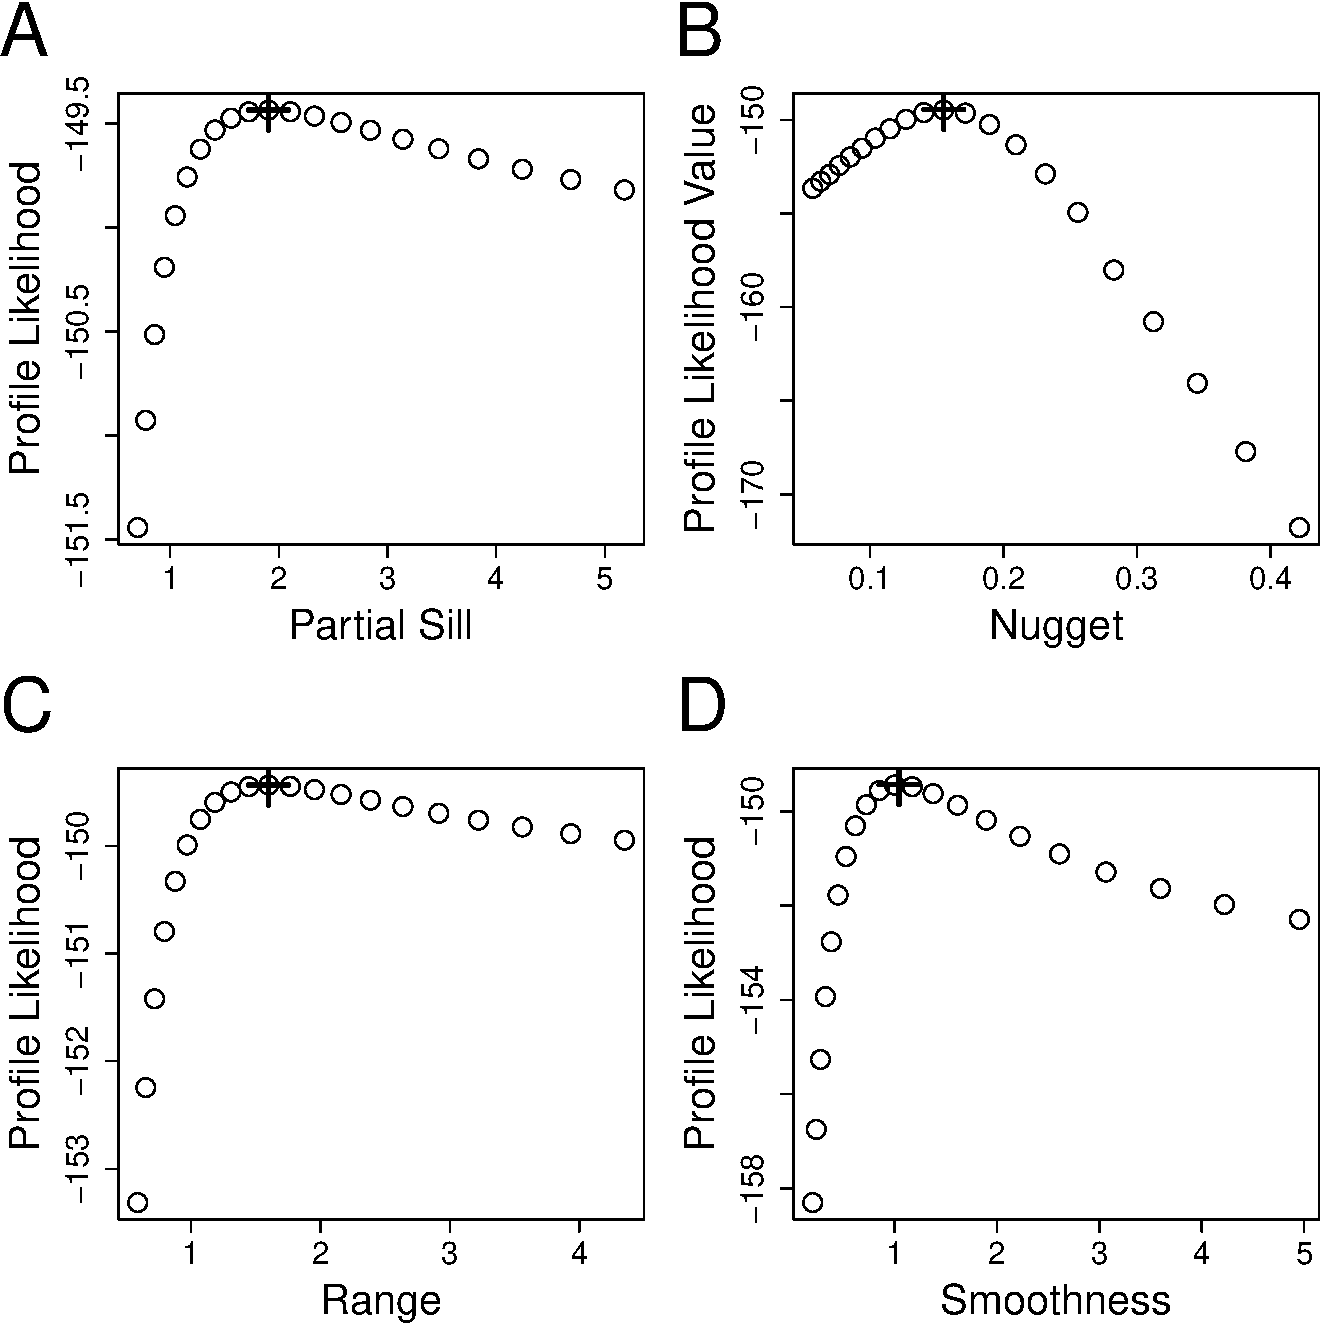
\includegraphics[width=.8\linewidth]{Matern_SO4}
  \end{center}
  \caption{Profile likehood for parameters in Matern model fitted to SO4 data with a constant mean. A. Partial Sill, B. Nugget, C. Range, and D. Smoothness.  For each parameter, the REML estimate is shown by a + and the value of the log likelihood at the REML estimate. \label{Fig:Matern_SO4}}
\end{figure}


Let us consider the Matern covariance function, which is very popular because it has an additional parameter that controls smoothness and differentiability of the surface that it produces.  In Table 6.1, this is denoted at $\theta_{3}$, and we will call it the smoothness parameter. If $\theta_{3} = 1/2$, then the Matern model is equivalent to the exponential model, if $\theta_{3} = 1$ is has been called the Whittle model, if $\theta_{3} = 3/2$ it is a radon model of order 2, if $\theta_{3} = 5/2$ it is a radon model of order 4, and as $\theta_{3} \rightarrow \infty$, the Matern model is equivalent to a Gaussian model.  In \texttt{spmodel}, the smoothness parameter is allowed to range from $1/5$ to 5.  For the Matern model, Figure~\ref{Fig:Matern_SO4}  shows the profile likelihood decreasing slowly as values for the partial sill and range increase beyond their REMLEs.  The nugget has a pronounced peak in the profile likelihood.  Some authors claim that the smoothness parameter for the Matern model is difficult to estimate, and they suggest either picking a single value, or pick several, and choose one based on the likelihood or other model selection criteria.  However, for these data, the smoothness parameter has a fairly well-defined maximum, and optimization had no issues.

\vspace{.3cm}

{\large \flushleft \textbf{9.10.2 Prediction of wet sulfate deposition}}

\vspace{.3cm}

We continue with our analysis from Section 8.8.3 of the clean wet sulfate deposition data in the conterminous U.S.  Our ultimate goal will be to create a map, with prediction intervals, on a grid of prediction locations across the whole U.S. that will help us assess the spatial patterns in wet sulfate deposition along with our confidence in those predictions.  We left some model selection choices open from Section 8.8.3 because predictive ability of those models will help in our selection process.  We will complete the analysis here, and begin with leave-one-out cross-validation (LOOCV).

LOOCV eliminates one datum at a time, using all of the rest of the data to predict the one that was removed.  There is a fast and a slow way to do this.  The slow way is to remove a datum and then re-estimate all of the parameters using ML or REML estimation each time.  However, with the removal of but a single datum, the parameter estimates change very little.  A fast way to achieve LOOCV is based on holding all parameters at their values as estimated by using all of the data, and then using results from partitioned matrices so that we only have to invert the covariance matrix once (which can be saved from the ML or REML estimation, so there is in fact no additional matrix inverses are required).  Recall from Section 5.6 that,
if a matrix is partitioned as,
$$
    \boldsymbol{\Sigma} = 
    \begin{bmatrix}
       \boldsymbol{\Sigma}_{11} & \boldsymbol{\Sigma}_{12} \\
       \boldsymbol{\Sigma}_{21} & \boldsymbol{\Sigma}_{22}
    \end{bmatrix}  \ \textrm{ and } \  
    \bSigma^{-1} = 
    \begin{bmatrix}
       \boldsymbol{\Sigma}^{11} & \boldsymbol{\Sigma}^{12} \\
       \boldsymbol{\Sigma}^{21} & \boldsymbol{\Sigma}^{22}
    \end{bmatrix}, 
$$
then 
$$
    \boldsymbol{\Sigma}_{11}^{-1} = \boldsymbol{\Sigma}^{11} - \boldsymbol{\Sigma}^{12} (\boldsymbol{\Sigma}^{22})^{-1} \boldsymbol{\Sigma}^{21}.
$$
Moreover, let us order the data such that the datum to be removed is last, so that $\boldsymbol{\Sigma}^{22}$ is a scalar, then the inverse of $\boldsymbol{\Sigma}^{22}$ is trivial and $\bSigma_{11} \upi$ can be computed rapidly. The main computational expense of kriging predictions rely on the inverse covariance matrix for the observed data, but in LOOCV that is given by $\bSigma_{11} \upi$, which is computed rapidly without any further matrix inverses if we already have $\bSigma \upi$. The only other quantity from $\boldsymbol{\Sigma}$ needed for prediction is the vector $\boldsymbol{\Sigma}_{12}$.  Conceptually, we just re-order the data, one at a time, putting the one to be removed last in the covariance matrices above, and that allows the predictions to be computed quickly.

Let $\hat{y}_{i} = \bar{u}$ from (9.2) be the $i$th predicted value using LOOCV where the $i$th datum has been removed, and let $\hat{v}_{i} = \sqrt{\var(\bar{u} - u)}$ from (9.3) be the $i$ prediction standard error.  Then we will consider two metrics to assess model performance.  One is the root-mean-squared prediction error (RMSPE), which we computed as
$$
\sqrt{\frac{1}{n}\sum_{i=1}^{n} (\hat{y}_{i} - y_{i})^{2} }.
$$
Models with lower RMSPE have better predictive performance.  The other metric is the 90\% prediction interval coverage, PIC90, which we computed as
$$
\frac{1}{n} \sum_{i=1}^{n} \mathcal{I}(\hat{y}_{i} - z_{1-\alpha/2}v_{i} \le y_{i} \le \hat{y}_{i} + z_{1-\alpha/2}v_{i}),
$$
where $\mathcal{I}(\cdot)$ is an indicator function, equal to 1 if its argument is true, and 0 otherwise, and $z_{1-\alpha/2}$ is a standard normal value below which contains $1-\alpha/2$ of the probability density.  We chose $\alpha = 0.1$ for PIC90, resulting in the familiar $z_{0.95} = 1.645$.

One problem with LOOCV is that it may be overly optimistic in assessing actual prediction.  A simple thought experiment reveals why.  Suppose 99 data locations were clustered very closely together, and another was separated from the cluster.  Then, for LOOCV, as we removed each datum from the cluster, we would have many nearby locations and get very precise predictions with small prediction standard errors, and they would swamp RMSPE and PIC90 if our overall goal was to predict in a region that was substantially larger than that enclosing the cluster of locations. The same is essentially true if all locations were pairs of locations that were very close to each other, but the pairs were scattered.  Still, under normal sampling scenarios, it can be a good way to evaluate models as they are all operating under the same sampling scheme.

A second way to use cross-validation is called $n$-fold cross-validation.  Here we divide the data into $n$ groups, and remove one whole group to be predicted -- this is often called the \textit{test} dataset.  The remaining data are called the \textit{training} dataset, and are used to fit a model and make predictions at the locations of the test dataset.  Then, the predictions at the locations for the test dataset can be compared to the actual values that were removed.  In fact, RMSPE and PIC90 can be computed for $n$-fold cross-validation in exactly the same way as for LOOCV, and to distinguish them, we use RMSPE$_{\textrm{Lo}}$ and PIC90$_{\textrm{Lo}}$ for LOOCV, and RMSPE$_{\textrm{Nf}}$ and PIC90$_{\textrm{Nf}}$ for $n$-fold cross-validation. With $n$-fold cross-validation we do not have to fit the model as many times, so we completely re-fit the model for each group that is removed.  Groups are often created randomly, and we will do it this way too.  If we want to get the best feel how well a model will interpolate, that includes even a bit of extrapolation at the edges, it is desirable to have just a few groups.  This may be more pessimistic about model performance than the real data because we are decreasing our sample sizes substantially.  Nevertheless, to examine both extremes, where LOOCV is overly optimistic, we used 3-fold cross-validation, which is overly pessimistic.  Because we created 3 groups randomly, we would like to ensure that our results do not depend too much on any particular randomized grouping.  Hence, we do 3-fold cross-validation 10 times, and average the results for RMSPE (by first averaging the mean-squared prediction error, and then taking the square root) and PIC90.

To further evaluate the models from from Section 8.8.3, we will consider LOOCV and 3-fold crossvalidation for polynomials with orders up to 5, again using the exponential autocovariance model.  RMSPE using LOOCV for the independence models generally goes down with increasing order of the polynomial surface (Figure~\ref{Fig:SO4_crossval}A), suggesting, like AIC and BIC, that among this set of models, a 4th or 5th order polynomial is best.  However, when it comes to predictive performance, the spatial models are much superior, having average deviations from true values of around 0.47 for lower order polynomials, versus approximately 0.53 for the higher order polynomials of the independence models, which translates to prediction intervals that are over 11\% shorter.  The problem of over-fitting polynomials is revealed more clearly by 3-fold cross-validation (Figure~\ref{Fig:SO4_crossval}C), where the RMSPE begins to increase rapidly for the independence models for the 5th order polynomial, and increases throughout for the spatial models. It also appears that for the spatial models in both Figure~\ref{Fig:SO4_crossval}A,C that REMLE is just slightly better than MLE.

\begin{figure}[H]
  \begin{center}
	    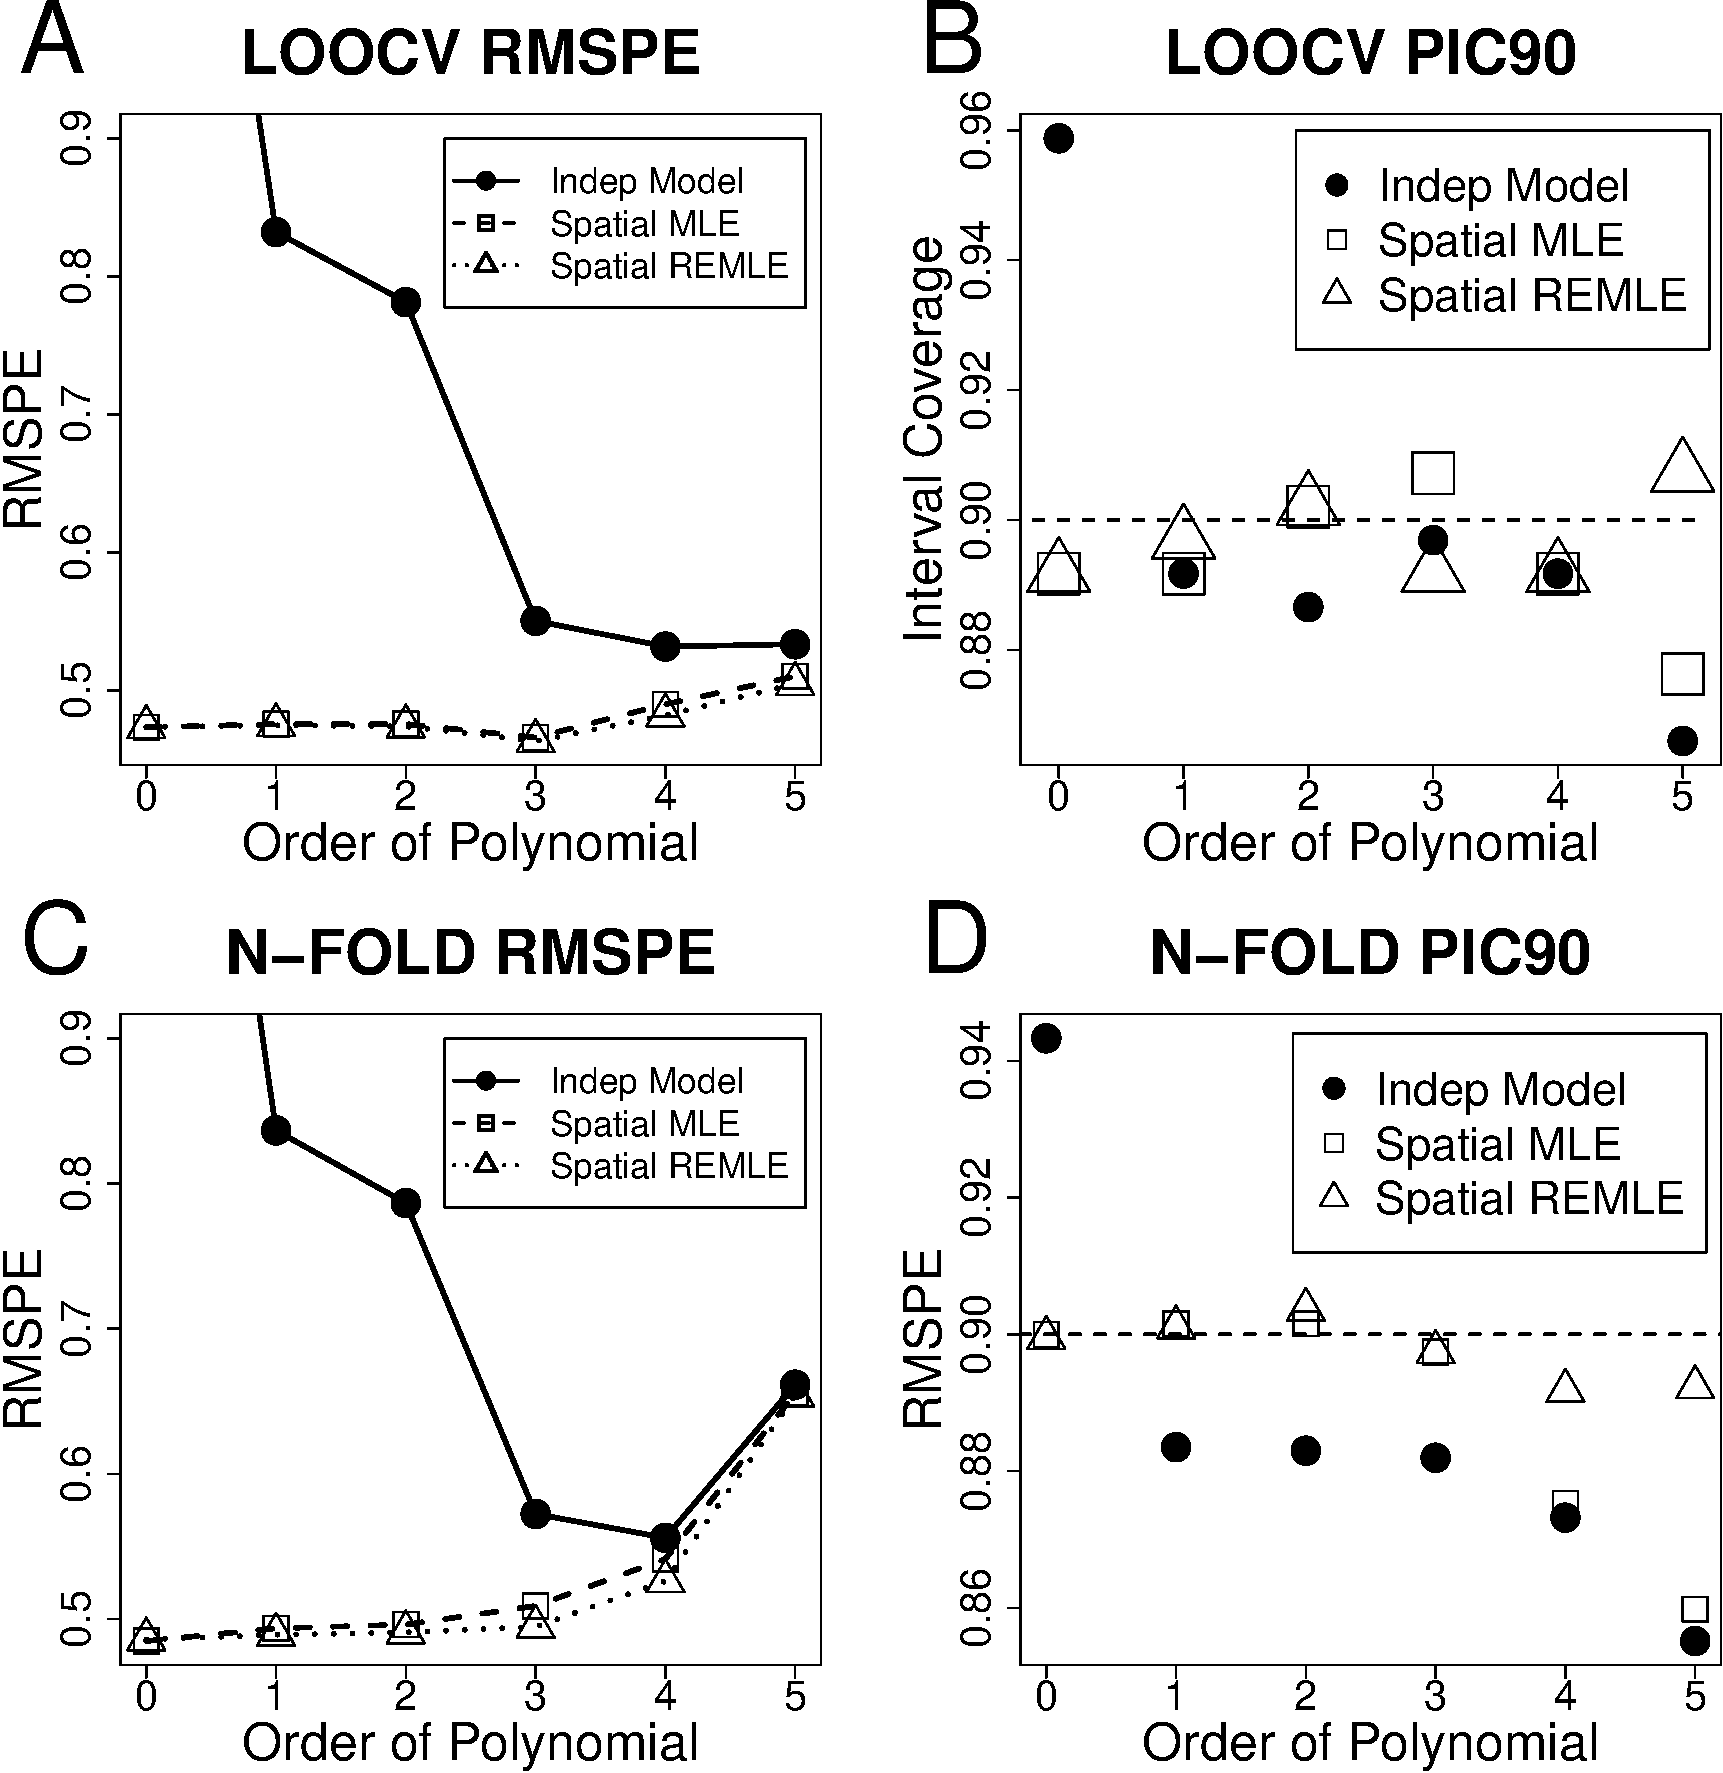
\includegraphics[width=.8\linewidth]{SO4_crossval}
  \end{center}
  \caption{Root-mean-squared prediction error (RMSPE) and 90\% prediction intervals coveraga (PIC90) using leave-one-out cross-validation (LOOCV) and 3-fold cross-validation for up to 5th order polynomial surfaces using the clean wet sulfate deposition data.  The spatial models were fit with an exponential autocovariate model using both MLE and REMLE. A. LOOCV RMSPE B. LOOCV PIC90 C. 3-fold RMSPE, and D. 3-fold PIC90. \label{Fig:SO4_crossval}}
\end{figure}

We want our prediction surfaces to be as precise as possible, but we also need to evaluate whether the estimated prediction standard-errors are valid.  By valid, we mean that a 90\% prediction interval should contain the true value 90\% of the time. For the independence models, that is approximately true for polynomial surfaces with orders 1 through 4, but the constant mean model is overly conservative (intervals that are larger than needed and thus containing the true values almost 96\% of the time, Figure~\ref{Fig:SO4_crossval}B, and 94\%, Figure~\ref{Fig:SO4_crossval}D), while the 5th order polynomial is overly optimistic (intervals that are too short and only contain the true value around 86\% of the time (Figure~\ref{Fig:SO4_crossval}B,D). The REML estimates are very close to the nominal value for all orders of the polynomial surface, while the ML estimates start to become too optimistic at order 4 using 3-fold cross-validation (Figure~\ref{Fig:SO4_crossval}D) and order 5 using LOOCV (Figure~\ref{Fig:SO4_crossval}B).

For the spatial models, based on BIC, LOOCV, and 3-fold cross-validation, there appears to be little reason to go beyond ordinary kriging.  However, we still need to choose an autocovariance model.  We fit most of the models in Table 6.1 using \texttt{spmodel}, and computed all of the model selection metrics discussed so far (Table~\ref{tab:ModelSelAutocov}).  With the exception of a few models like wave and J-Bessel, all models performed similarly. Also note that with a constant mean model, there was very little difference between LOOCV and 3-fold cross-validation. The spherical model is just slightly better than most others based on AIC, BIC, and RMSPE.  It also appears to have appropriate prediction interval coverage, so we will choose the spherical model for further analyses.
\begin{table}[h] 
				\caption{Performance metrics for various covariance functions used with a constant mean model fit with REMLE for the clean wet sulfate data. \label{tab:ModelSelAutocov}}
\begin{center}
\begin{tabular}{c|rrrrrrr}
  \hline
  \hline
  Model & m2LL & AIC & BIC & RMSPE$_{\textrm{Lo}}$ & RMSPE$_{\textrm{Nf}}$ & PIC90$_{\textrm{Lo}}$ & PIC90$_{\textrm{Nf}}$ \\
	\hline
  \hline
exponential & 302.4 & 308.4 & 318.2 & 0.473 & 0.473 & 0.892 & 0.907 \\ 
  spherical & 298.8 & 304.8 & 314.6 & 0.469 & 0.470 & 0.887 & 0.902 \\ 
  gaussian & 308.5 & 314.5 & 324.3 & 0.487 & 0.490 & 0.871 & 0.907 \\ 
  circular & 302.6 & 308.6 & 318.4 & 0.474 & 0.480 & 0.892 & 0.897 \\ 
  pentaspherical & 299.5 & 305.5 & 315.3 & 0.470 & 0.470 & 0.887 & 0.902 \\ 
  wave & 323.4 & 329.4 & 339.2 & 0.510 & 0.515 & 0.902 & 0.892 \\ 
  jbessel & 328.9 & 334.9 & 344.7 & 0.530 & 0.527 & 0.902 & 0.892 \\ 
  gravity & 301.2 & 307.2 & 317.0 & 0.477 & 0.479 & 0.887 & 0.892 \\ 
  rquad & 302.1 & 308.1 & 317.9 & 0.478 & 0.480 & 0.881 & 0.897 \\ 
  magnetic & 303.0 & 309.0 & 318.8 & 0.479 & 0.481 & 0.876 & 0.897 \\ 
  matern & 303.9 & 311.9 & 324.9 & 0.481 & 0.483 & 0.871 & 0.897 \\ 
  cauchy & 300.4 & 308.4 & 321.5 & 0.475 & 0.481 & 0.887 & 0.892 \\ 
  pexponential & 298.3 & 306.3 & 319.4 & 0.473 & 0.471 & 0.887 & 0.902 \\
   \hline
	\hline
\end{tabular}
\end{center}
\end{table}

Now we are ready to make maps of wet sulfate deposition across the U.S.  We created an evenly spaced grid of points and clipped them to the boundaries of the continental U.S., resulting in 3663 prediction locations.  We used 5 different models to illustrate various features of the resulting maps. Figure~\ref{Fig:SO4_predMaps}A shows predictions for a 4th order polynomial assuming independent errors. The prediction standard errors show the typical pattern for regression models, where the variance is smallest near the mean of the explanatory variables (spatial coordinates in this case).  Hence, the prediction standard errors are smallest near the center of the country, somewhat weighted by the fact that there are more samples in the northeast (Figure~\ref{Fig:SO4_predMaps}B). For this 4th order polynomial model, standard errors are marginally reliable, as shown by PIC90 from LOOCV and 3-fold cross-validations. 

The spatial model with a constant mean and a spherical autocovariance is a more flexible surface than the polynomial surface (Figure~\ref{Fig:SO4_predMaps}C).  For example, there is a small area of higher sulfate deposition along the middle southern boarder of the U.S. near New Orleans, in the state of Louisiana, which is shaped like a boot. The higher concentrations are apparent in the ``toe'' of the boot.  An autocorrelated surface is more flexible to take on smaller fluctuations like this.  The map of prediction standard errors (Figure~\ref{Fig:SO4_predMaps}D) exhibits a ``bull's eye'' pattern around locations with observed data, which is characteristic of many of the autocovariance models, this map is very different then the smooth surface in Figure~\ref{Fig:SO4_predMaps}B.  Overall, the estimated prediction standard errors in Figure~\ref{Fig:SO4_predMaps}D are significantly lower than those of Figure~\ref{Fig:SO4_predMaps}B, which we we believe to be valid based on our cross-validation analysis of these data. 

We also show that, while we chose the spherical model, many of the other covariance functions would give very similar results (e.g., the exponential model in Figures~\ref{Fig:SO4_predMaps}E,F. There is some advice in the literature suggesting that the choice of which autocovariance function is not that important, at least not in comparison to the important choice a spatial model versus the model assuming independent errors.  To a certain extent, this is even true for these data when comparing the spherical model with a constant mean (Figures~\ref{Fig:SO4_predMaps}C,D) to a spherical model with a 3rd-order polynomial on the coordinates as fixed effects (Figures~\ref{Fig:SO4_predMaps}G,H), where the prediction standard errors are somewhat more diffuse, but the prediction maps are virtually identical.

However, we suggest that for a practical analysis several models should be tried to see if and where they differ.  One model that is often very different from the others is the Gaussian autocovariance model.  It creates very smooth surfaces, and Figure~\ref{Fig:SO4_predMaps}I shows that the area of higher concentration in the toe of Louisiana (Figure~\ref{Fig:SO4_predMaps}C,E,G) is not apparent when using this model, and the prediction standard errors change more gradually (Figure~\ref{Fig:SO4_predMaps}J), rather than having the bull's eye effect.  Generally, autocovariance models that are flat near the origin, and having a sigmoid shape, will behave more like Figures~\ref{Fig:SO4_predMaps}I,J, while those that drop rapidly and linearly near the origin will behave more like Figures~\ref{Fig:SO4_predMaps}C,D.

\begin{figure}[H]
  \begin{center}
	    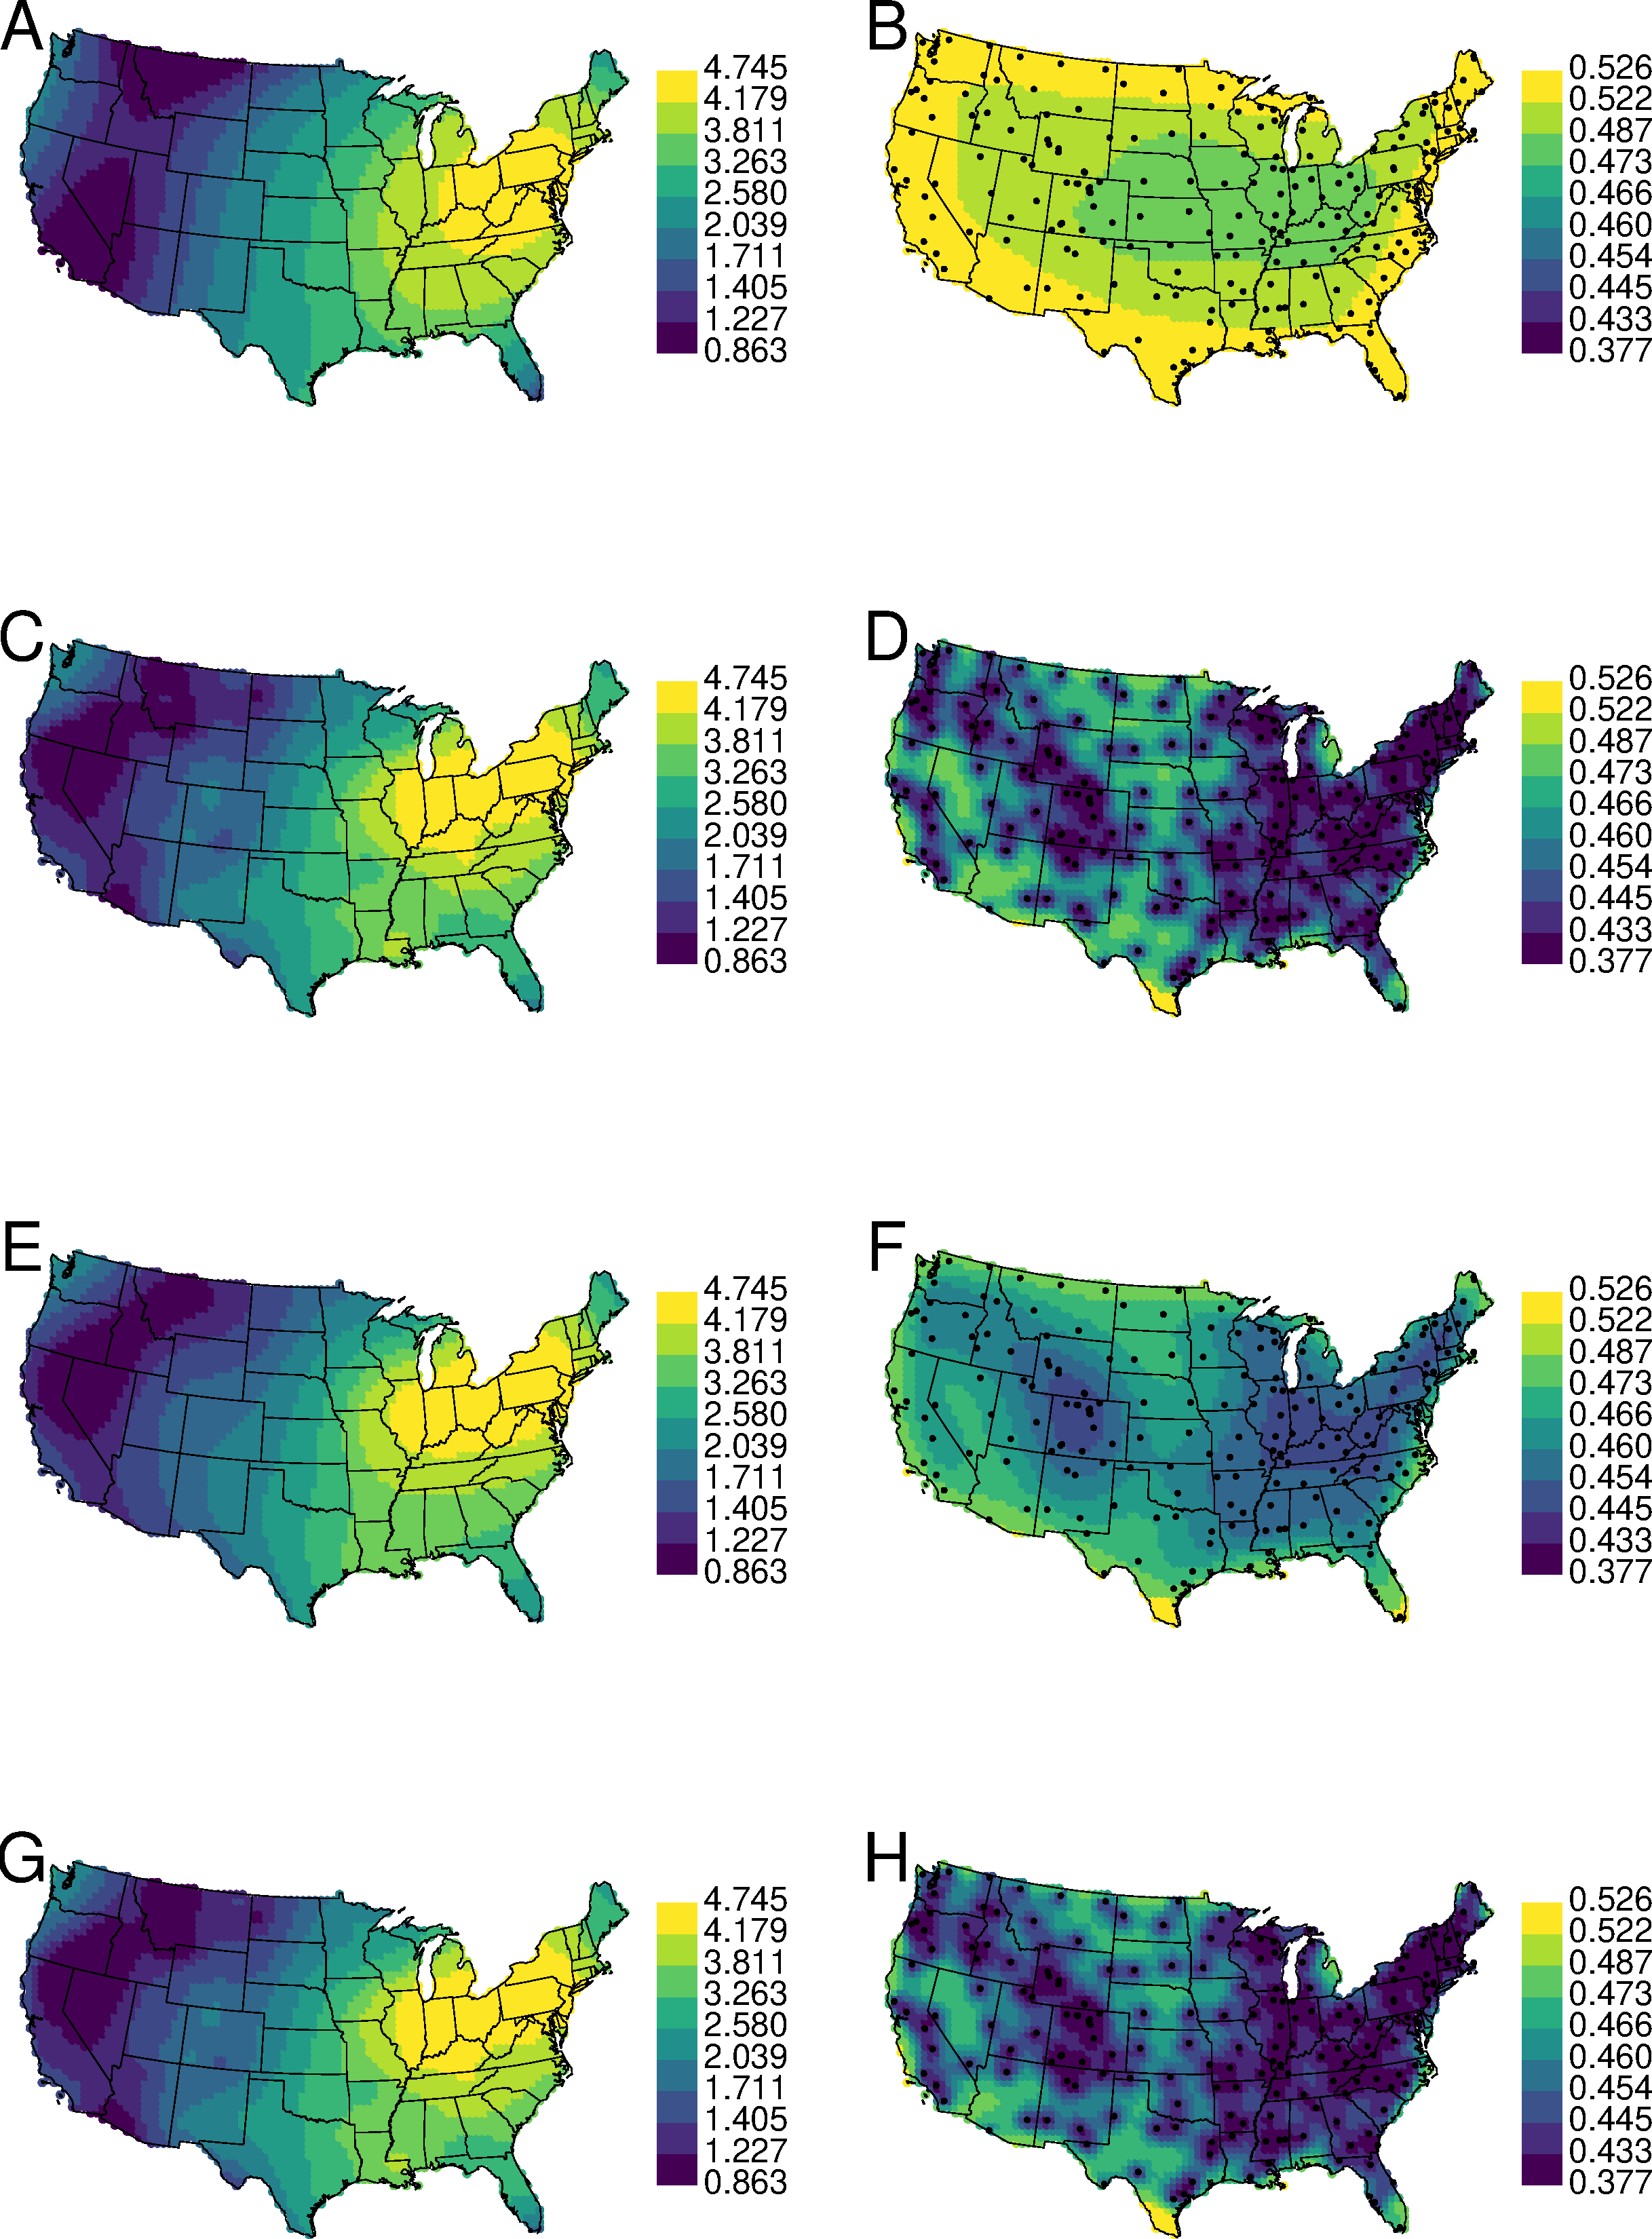
\includegraphics[width=.8\linewidth]{SO4_Prediction_Maps}
  \end{center}
  \caption{Prediction maps (left column) and prediction standard errors (right column) for a variety of models. A-B Fourth-order polynomial assuming independent errors, C-D constant mean spherical model, E-F constant mean exponential model, G-H Third-order polynomial spherical model, I-J constant mean Gaussian model. \label{Fig:SO4_predMaps}}
\end{figure}

%%%%%%%%%%%%%%%%%%%%%%%%%%%%%%%%%%%%%%%%%%%%%%%%%%%%%%%%%%%%%%%%%%%%%%%%%%%%%%%%%%
%%%%%%%%%%%%%%%%%%%%%%%%%%%%%%%%%%%%%%%%%%%%%%%%%%%%%%%%%%%%%%%%%%%%%%%%%%%%%%%%%%
%                BIBLIOGRAPHY
%%%%%%%%%%%%%%%%%%%%%%%%%%%%%%%%%%%%%%%%%%%%%%%%%%%%%%%%%%%%%%%%%%%%%%%%%%%%%%%%%%
%%%%%%%%%%%%%%%%%%%%%%%%%%%%%%%%%%%%%%%%%%%%%%%%%%%%%%%%%%%%%%%%%%%%%%%%%%%%%%%%%%

%\bibliographystyle{consbiol}
\bibliographystyle{/mnt/ExtraDrive1/Work/shTex/asa}
\bibliography{DaleChap883.bib}
%\bibliographystyle{/home/jay/Data/shTex/shTex/asa}
%\bibliography{/home/jay/Data/shTex/shTex/StatBibTex.bib}




\end{document}

